% Options for packages loaded elsewhere
\PassOptionsToPackage{unicode}{hyperref}
\PassOptionsToPackage{hyphens}{url}
\PassOptionsToPackage{dvipsnames,svgnames,x11names}{xcolor}
%
\documentclass[
  ignorenonframetext,
  aspectratio=169,
]{beamer}
\usepackage{pgfpages}
\setbeamertemplate{caption}[numbered]
\setbeamertemplate{caption label separator}{: }
\setbeamercolor{caption name}{fg=normal text.fg}
\beamertemplatenavigationsymbolshorizontal
% Prevent slide breaks in the middle of a paragraph
\widowpenalties 1 10000
\raggedbottom
\setbeamertemplate{part page}{
  \centering
  \begin{beamercolorbox}[sep=16pt,center]{part title}
    \usebeamerfont{part title}\insertpart\par
  \end{beamercolorbox}
}
\setbeamertemplate{section page}{
  \centering
  \begin{beamercolorbox}[sep=12pt,center]{part title}
    \usebeamerfont{section title}\insertsection\par
  \end{beamercolorbox}
}
\setbeamertemplate{subsection page}{
  \centering
  \begin{beamercolorbox}[sep=8pt,center]{part title}
    \usebeamerfont{subsection title}\insertsubsection\par
  \end{beamercolorbox}
}
\AtBeginPart{
  \frame{\partpage}
}
\AtBeginSection{
  \ifbibliography
  \else
    \frame{\sectionpage}
  \fi
}
\AtBeginSubsection{
  \frame{\subsectionpage}
}

\usepackage{amsmath,amssymb}
\usepackage{iftex}
\ifPDFTeX
  \usepackage[T1]{fontenc}
  \usepackage[utf8]{inputenc}
  \usepackage{textcomp} % provide euro and other symbols
\else % if luatex or xetex
  \usepackage{unicode-math}
  \defaultfontfeatures{Scale=MatchLowercase}
  \defaultfontfeatures[\rmfamily]{Ligatures=TeX,Scale=1}
\fi
\usetheme[]{Hannover}
\usecolortheme{rose}
\usepackage[]{libertinus}
\ifPDFTeX\else  
    % xetex/luatex font selection
\fi
% Use upquote if available, for straight quotes in verbatim environments
\IfFileExists{upquote.sty}{\usepackage{upquote}}{}
\IfFileExists{microtype.sty}{% use microtype if available
  \usepackage[]{microtype}
  \UseMicrotypeSet[protrusion]{basicmath} % disable protrusion for tt fonts
}{}
\makeatletter
\@ifundefined{KOMAClassName}{% if non-KOMA class
  \IfFileExists{parskip.sty}{%
    \usepackage{parskip}
  }{% else
    \setlength{\parindent}{0pt}
    \setlength{\parskip}{6pt plus 2pt minus 1pt}}
}{% if KOMA class
  \KOMAoptions{parskip=half}}
\makeatother
\usepackage{xcolor}
\newif\ifbibliography
\setlength{\emergencystretch}{3em} % prevent overfull lines
\setcounter{secnumdepth}{-\maxdimen} % remove section numbering


\providecommand{\tightlist}{%
  \setlength{\itemsep}{0pt}\setlength{\parskip}{0pt}}\usepackage{longtable,booktabs,array}
\usepackage{calc} % for calculating minipage widths
\usepackage{caption}
% Make caption package work with longtable
\makeatletter
\def\fnum@table{\tablename~\thetable}
\makeatother
\usepackage{graphicx}
\makeatletter
\def\maxwidth{\ifdim\Gin@nat@width>\linewidth\linewidth\else\Gin@nat@width\fi}
\def\maxheight{\ifdim\Gin@nat@height>\textheight\textheight\else\Gin@nat@height\fi}
\makeatother
% Scale images if necessary, so that they will not overflow the page
% margins by default, and it is still possible to overwrite the defaults
% using explicit options in \includegraphics[width, height, ...]{}
\setkeys{Gin}{width=\maxwidth,height=\maxheight,keepaspectratio}
% Set default figure placement to htbp
\makeatletter
\def\fps@figure{htbp}
\makeatother
% definitions for citeproc citations
\NewDocumentCommand\citeproctext{}{}
\NewDocumentCommand\citeproc{mm}{%
  \begingroup\def\citeproctext{#2}\cite{#1}\endgroup}
\makeatletter
 % allow citations to break across lines
 \let\@cite@ofmt\@firstofone
 % avoid brackets around text for \cite:
 \def\@biblabel#1{}
 \def\@cite#1#2{{#1\if@tempswa , #2\fi}}
\makeatother
\newlength{\cslhangindent}
\setlength{\cslhangindent}{1.5em}
\newlength{\csllabelwidth}
\setlength{\csllabelwidth}{3em}
\newenvironment{CSLReferences}[2] % #1 hanging-indent, #2 entry-spacing
 {\begin{list}{}{%
  \setlength{\itemindent}{0pt}
  \setlength{\leftmargin}{0pt}
  \setlength{\parsep}{0pt}
  % turn on hanging indent if param 1 is 1
  \ifodd #1
   \setlength{\leftmargin}{\cslhangindent}
   \setlength{\itemindent}{-1\cslhangindent}
  \fi
  % set entry spacing
  \setlength{\itemsep}{#2\baselineskip}}}
 {\end{list}}
\usepackage{calc}
\newcommand{\CSLBlock}[1]{\hfill\break\parbox[t]{\linewidth}{\strut\ignorespaces#1\strut}}
\newcommand{\CSLLeftMargin}[1]{\parbox[t]{\csllabelwidth}{\strut#1\strut}}
\newcommand{\CSLRightInline}[1]{\parbox[t]{\linewidth - \csllabelwidth}{\strut#1\strut}}
\newcommand{\CSLIndent}[1]{\hspace{\cslhangindent}#1}

\makeatletter
\@ifpackageloaded{caption}{}{\usepackage{caption}}
\AtBeginDocument{%
\ifdefined\contentsname
  \renewcommand*\contentsname{Table of contents}
\else
  \newcommand\contentsname{Table of contents}
\fi
\ifdefined\listfigurename
  \renewcommand*\listfigurename{List of Figures}
\else
  \newcommand\listfigurename{List of Figures}
\fi
\ifdefined\listtablename
  \renewcommand*\listtablename{List of Tables}
\else
  \newcommand\listtablename{List of Tables}
\fi
\ifdefined\figurename
  \renewcommand*\figurename{Figure}
\else
  \newcommand\figurename{Figure}
\fi
\ifdefined\tablename
  \renewcommand*\tablename{Table}
\else
  \newcommand\tablename{Table}
\fi
}
\@ifpackageloaded{float}{}{\usepackage{float}}
\floatstyle{ruled}
\@ifundefined{c@chapter}{\newfloat{codelisting}{h}{lop}}{\newfloat{codelisting}{h}{lop}[chapter]}
\floatname{codelisting}{Listing}
\newcommand*\listoflistings{\listof{codelisting}{List of Listings}}
\makeatother
\makeatletter
\makeatother
\makeatletter
\@ifpackageloaded{caption}{}{\usepackage{caption}}
\@ifpackageloaded{subcaption}{}{\usepackage{subcaption}}
\makeatother
\ifLuaTeX
  \usepackage{selnolig}  % disable illegal ligatures
\fi
\usepackage{bookmark}

\IfFileExists{xurl.sty}{\usepackage{xurl}}{} % add URL line breaks if available
\urlstyle{same} % disable monospaced font for URLs
\hypersetup{
  pdftitle={Belonging and Exclusion},
  pdfauthor={Usman Afzali, PhD - Postdoctoral Fellow},
  colorlinks=true,
  linkcolor={Maroon},
  filecolor={Maroon},
  citecolor={Blue},
  urlcolor={Blue},
  pdfcreator={LaTeX via pandoc}}

\title{Belonging and Exclusion}
\subtitle{The Psychology of Identity Crisis in a Diverse World}
\author{Usman Afzali, PhD - Postdoctoral Fellow}
\date{2024-05-31}
\institute{University of Canterbury}
\logo{
\includegraphics{mds.png}}

\begin{document}
\frame{\titlepage}

\begin{frame}
\begin{figure}

\begin{minipage}{\linewidth}
\begin{center}

\includegraphics[width=0.6\textwidth,height=\textheight]{figs/mds.png}
\end{center}

\includegraphics{figs/sponsors.png}\end{minipage}%

\end{figure}%
\end{frame}

\begin{frame}{Outline}
\phantomsection\label{outline}
\begin{itemize}
\tightlist
\item
  Social perspective
\item
  Developmental perspective
\item
  Identity denial
\item
  Negative consequences
\item
  What to do?
\end{itemize}
\end{frame}

\begin{frame}
\textbf{What is your perception from the term \emph{``identity''}?}
\end{frame}

\section{How is identity formed
socially?}\label{how-is-identity-formed-socially}

\begin{frame}{Identity formation}
\phantomsection\label{identity-formation}
\begin{itemize}[<+->]
\tightlist
\item
  People all over the world believe that their own nation, culture,
  language, and religion are better and more deserving than others.
\item
  But why?
\item
  Henri Tajfel (1971)
\end{itemize}
\end{frame}

\begin{frame}
Henri Tajfel 1919 - 1982. From Wikipedia (The Free Encyclopedia)

\begin{center}
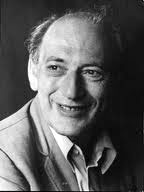
\includegraphics{figs/Henri_Tajfel.jpg}
\end{center}
\end{frame}

\begin{frame}{Social experiment}
\phantomsection\label{social-experiment}
\begin{columns}[c,totalwidth=8em]
\begin{column}{0.4\textwidth}
\begin{itemize}[<+->]
\tightlist
\item
  \textbf{Task 1}: Estimate the number of dots on each slide
\item
  \textbf{Outcome}: \emph{``Over-estimators''} and
  \emph{``under-estimators''}
\item
  Divided into two random groups
\item
  \textbf{Task 2}: Allocate points to other participants that can be
  cashed for money.
\end{itemize}
\end{column}

\begin{column}{0.6\textwidth}

\includegraphics{figs/tajfel.png}
\end{column}
\end{columns}
\end{frame}

\begin{frame}[fragile]{Findings}
\phantomsection\label{findings}
\begin{itemize}[<+->]
\tightlist
\item
  Allocated \textbf{more} points to members of their own group than to
  members of the other group.
\item
  \emph{Ingroup favouritism} (discrimination)
\item
  Replicated in many countries
\item
  \texttt{Minimal\ Groups\ Paradigm}
\end{itemize}
\end{frame}

\begin{frame}{The need for self-esteem}
\phantomsection\label{the-need-for-self-esteem}
Kassin et al.~(2021)

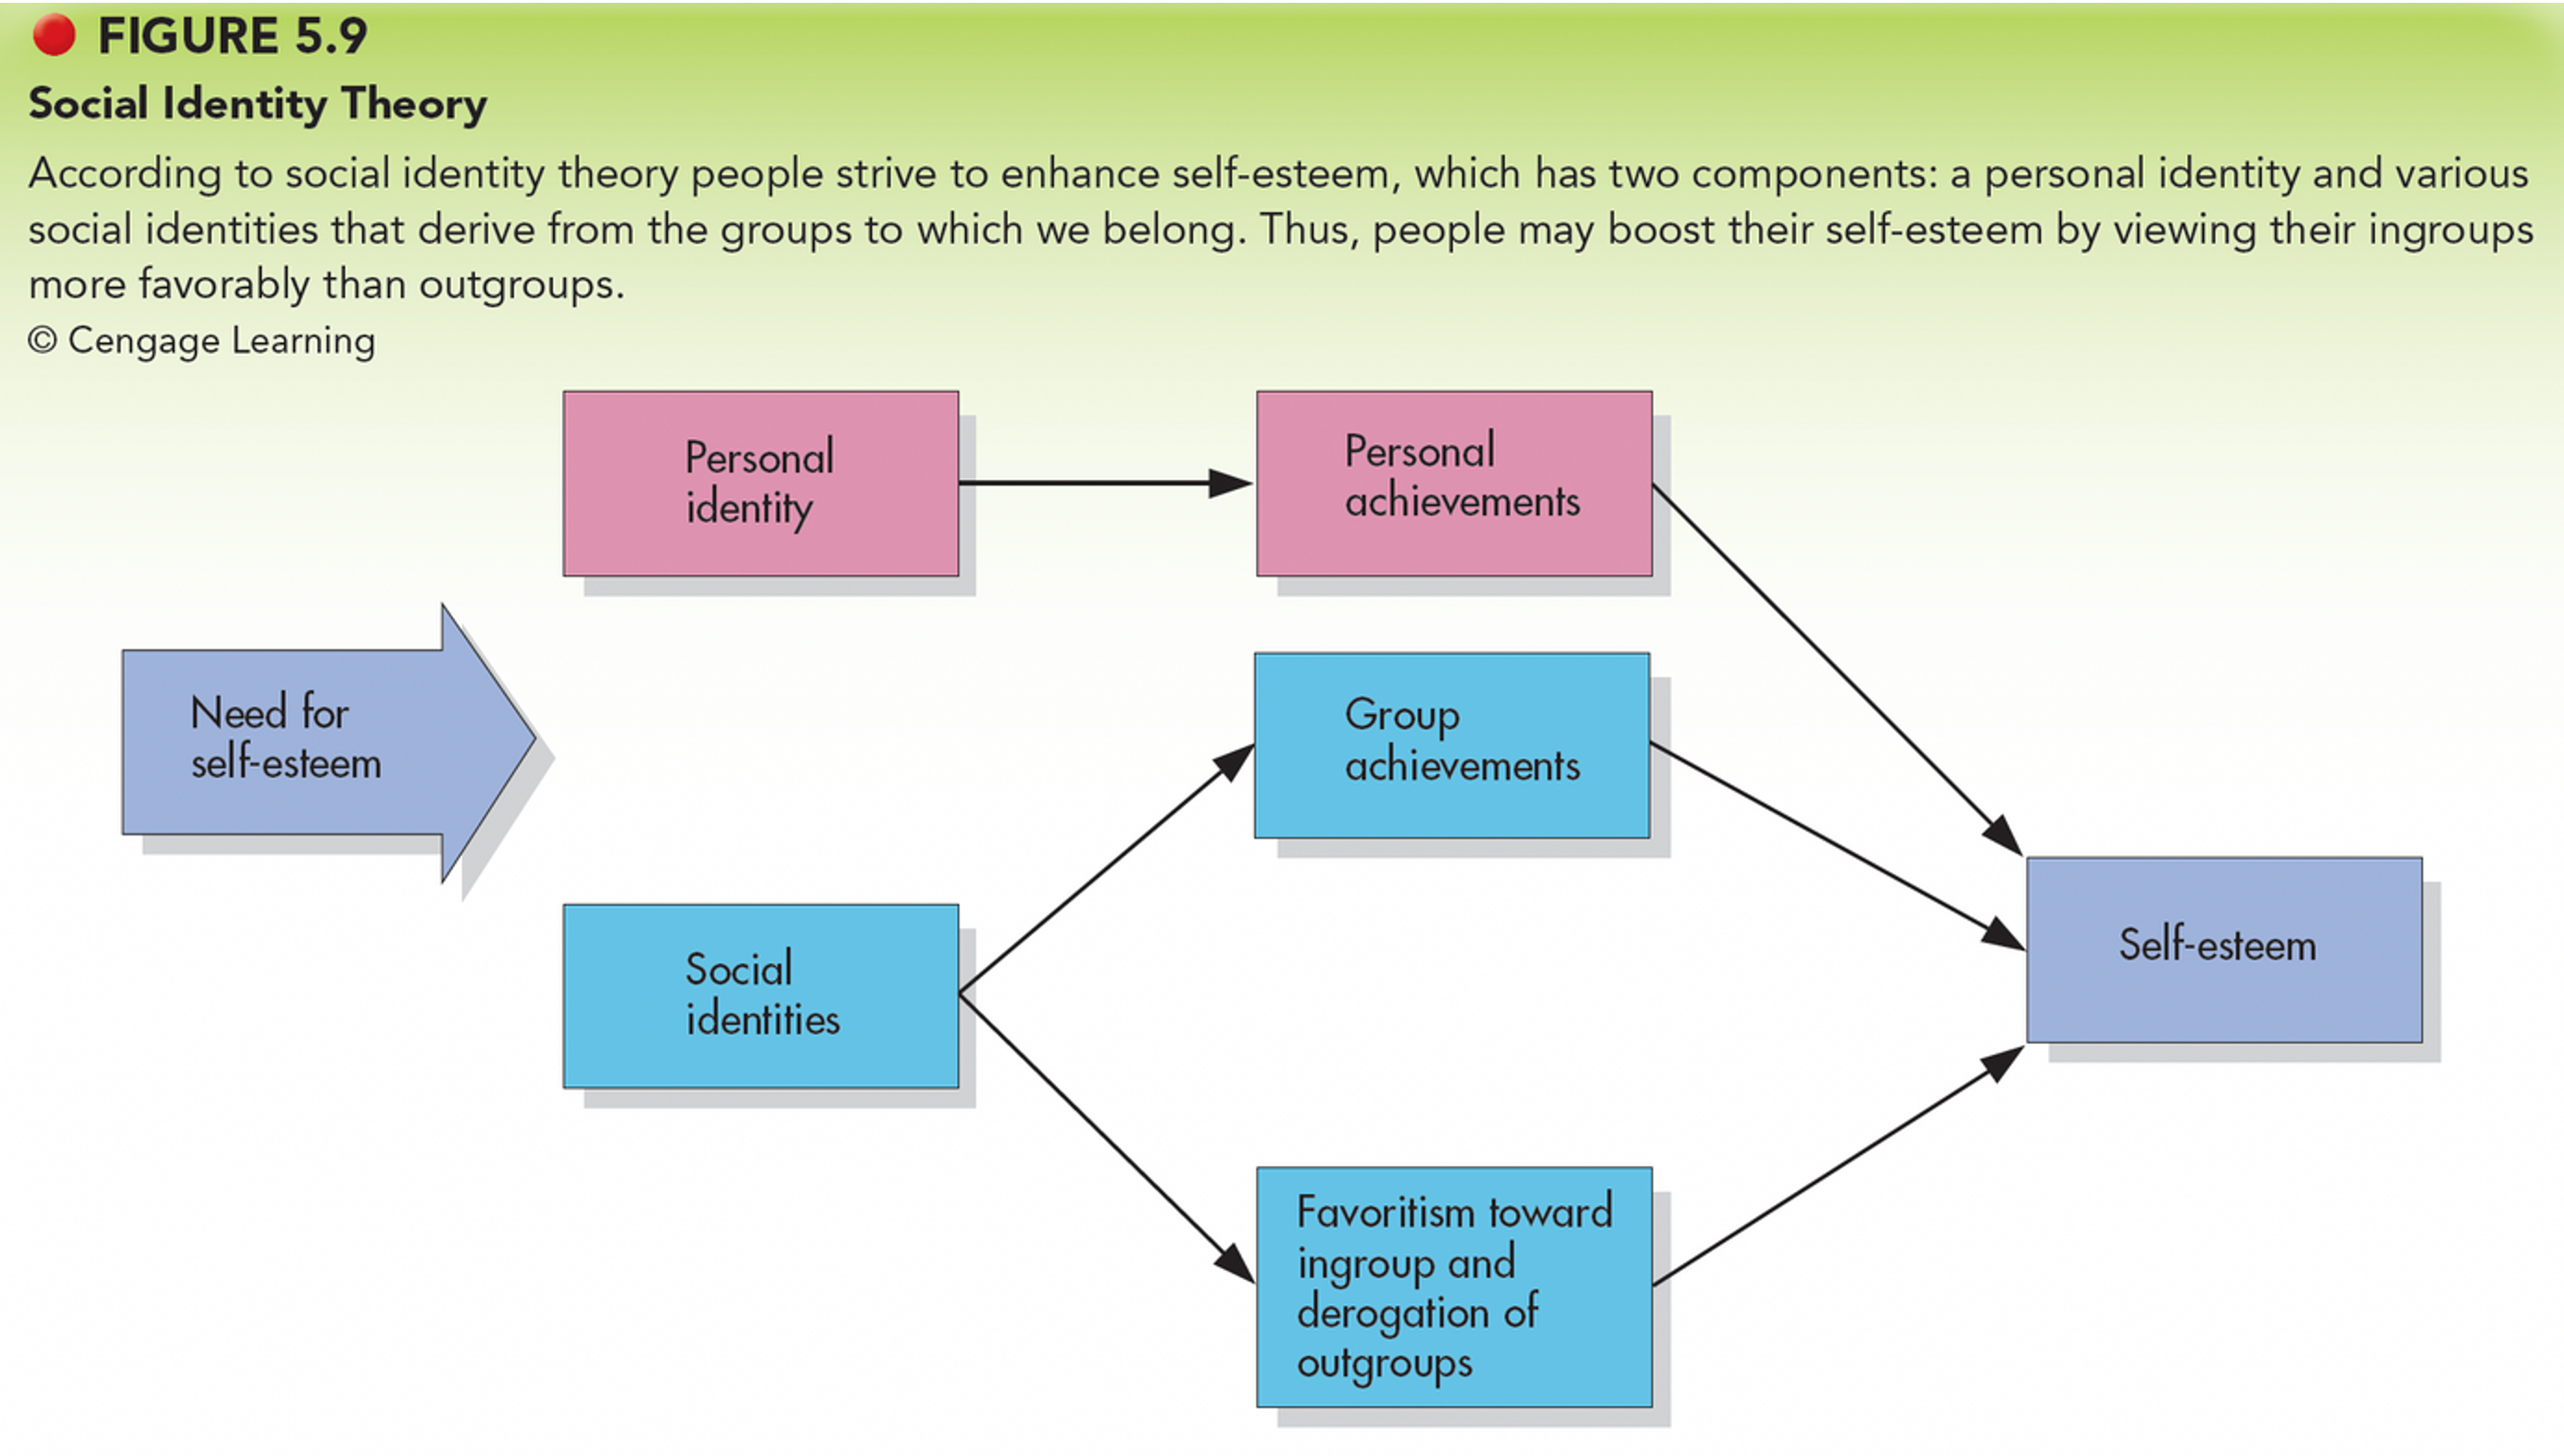
\includegraphics[width=0.9\textwidth,height=\textheight]{figs/selfesteem.png}
\end{frame}

\begin{frame}
\begin{itemize}[<+->]
\tightlist
\item
  \textbf{Advantage}: Derive pride from our connections
\item
  \textbf{Disadvantage}: The need to belittle \emph{``them''} in order
  to feel secure about \emph{``us''}.
\item
  Examples: Religious fervor, racial and ethnic conceit, aggressive
  nationalism, and even gossiping (Bosson et al. 2006; Weaver and Bosson
  2011)
\item
  When people shared negative attitudes about a third party, they felt
  closer to each other.
\end{itemize}
\end{frame}

\begin{frame}{A scenario}
\phantomsection\label{a-scenario}
\begin{itemize}[<+->]
\tightlist
\item
  In New Zealand, as in many other parts of the world, Muslims often
  face stereotypes and prejudices due to their religion, culture, or
  appearance. Islamophobia, or fear and hostility toward Islam and
  Muslims, can be pervasive in society and can manifest in various
  forms, such as discrimination, harassment, or even violence.
\item
  Now, suppose an individual in New Zealand experiences a threat to
  their self-esteem, such as being criticized by colleagues at work or
  feeling excluded in a social setting. In response to this threat, they
  may seek ways to restore their sense of self-worth or superiority.
  Unfortunately, in some cases, individuals may resort to derogating
  others, including Muslims, as a means of boosting their own
  self-esteem.
\end{itemize}
\end{frame}

\begin{frame}
\begin{itemize}[<+->]
\tightlist
\item
  For example, this person might start expressing or endorsing negative
  stereotypes about Muslims, such as portraying them as
  \emph{terrorists}, \emph{backward}, or \emph{incompatible} with
  Western values. By doing so, they may attempt to reaffirm their own
  \emph{identity} or sense of \emph{belonging} within the dominant
  culture, thus temporarily alleviating their feelings of
  \emph{insecurity} or \emph{inferiority}.
\item
  By linking the individual's feelings of insecurity or threat in social
  or professional settings to the broader context of Islamophobia in New
  Zealand, we can illustrate how the self-esteem maintenance model (Fein
  and Spencer 1997) may play out in real-life situations, where
  individuals derogate members of stereotyped groups, such as Muslims,
  to cope with their own insecurities.
\end{itemize}
\end{frame}

\begin{frame}
\textbf{People all over the world believe that their own nation,
culture, language, and religion are better and more deserving than
others.}
\end{frame}

\begin{frame}[fragile]
\textbf{But wait\ldots{} \texttt{When} do we start thinking about
identity?}
\end{frame}

\section{Identity development}\label{identity-development}

\begin{frame}{Erik Erikson}
\phantomsection\label{erik-erikson}
1902 - 1994. From Wikipedia (The Free Encyclopedia)

\begin{center}
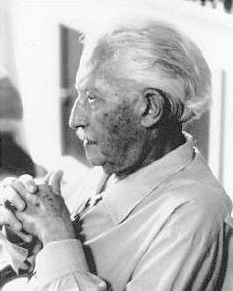
\includegraphics{figs/Erik_Erikson.jpg}
\end{center}
\end{frame}

\begin{frame}{Psychosocial theory of human development}
\phantomsection\label{psychosocial-theory-of-human-development}
\begin{itemize}[<+->]
\tightlist
\item
  Stages of development
\item
  Each stage represents a psychosocial crisis
\item
  ``Human \emph{personality} in principle develops according to steps
  predetermined in the growing person's readiness to be driven toward,
  to be aware of, and to interact with a widening social radius.'' -- c.
  1963
\end{itemize}
\end{frame}

\begin{frame}{Psychosocial theory of human development}
\phantomsection\label{psychosocial-theory-of-human-development-1}
Weiten (2013)
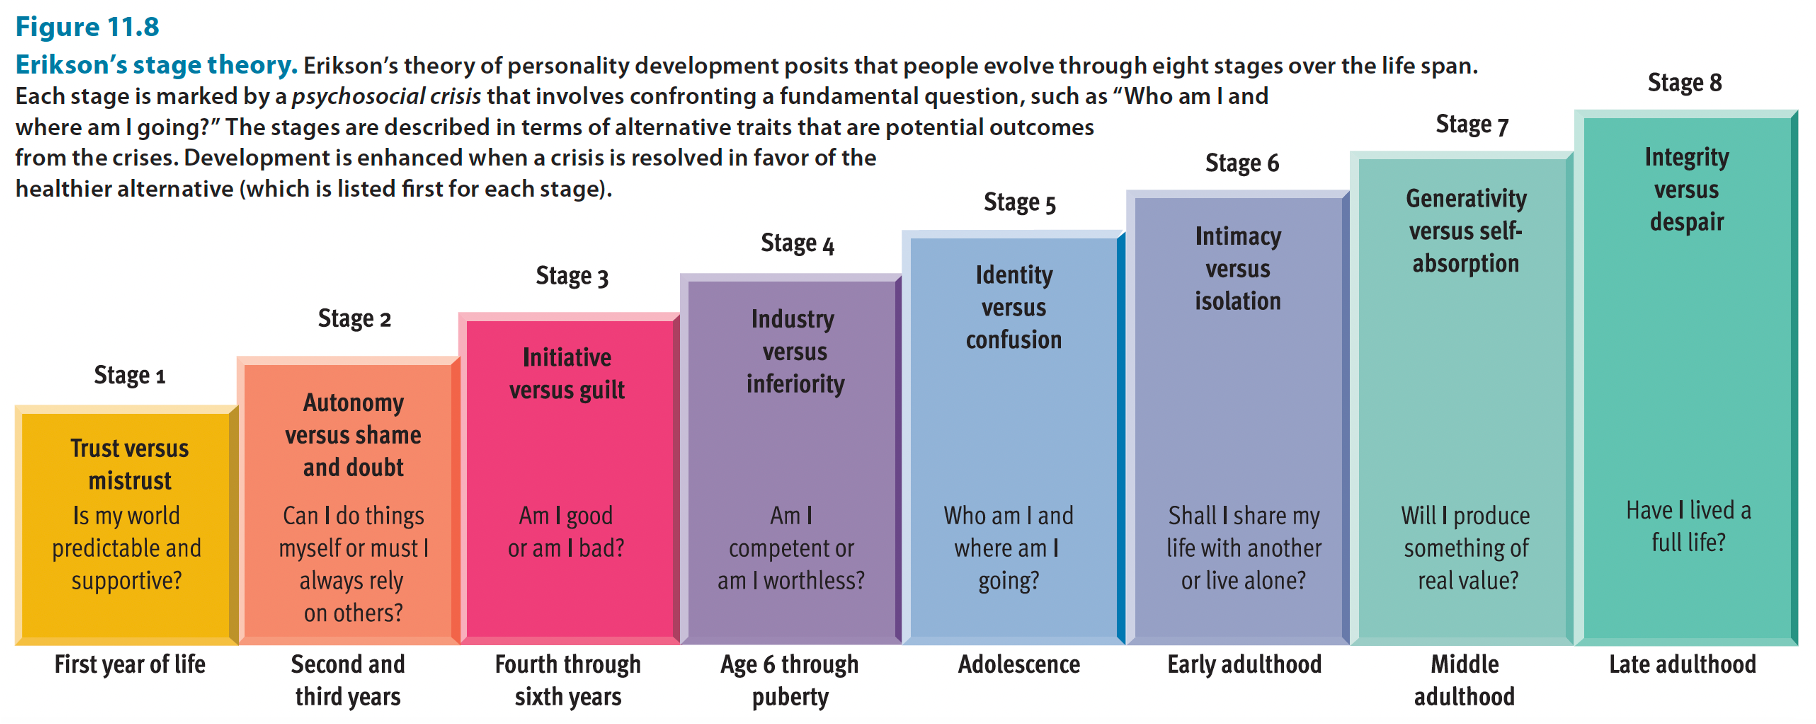
\includegraphics[width=0.9\textwidth,height=\textheight]{figs/stages.png}
\end{frame}

\begin{frame}{Marcia's identity statuses}
\phantomsection\label{marcias-identity-statuses}
Weiten (2013) 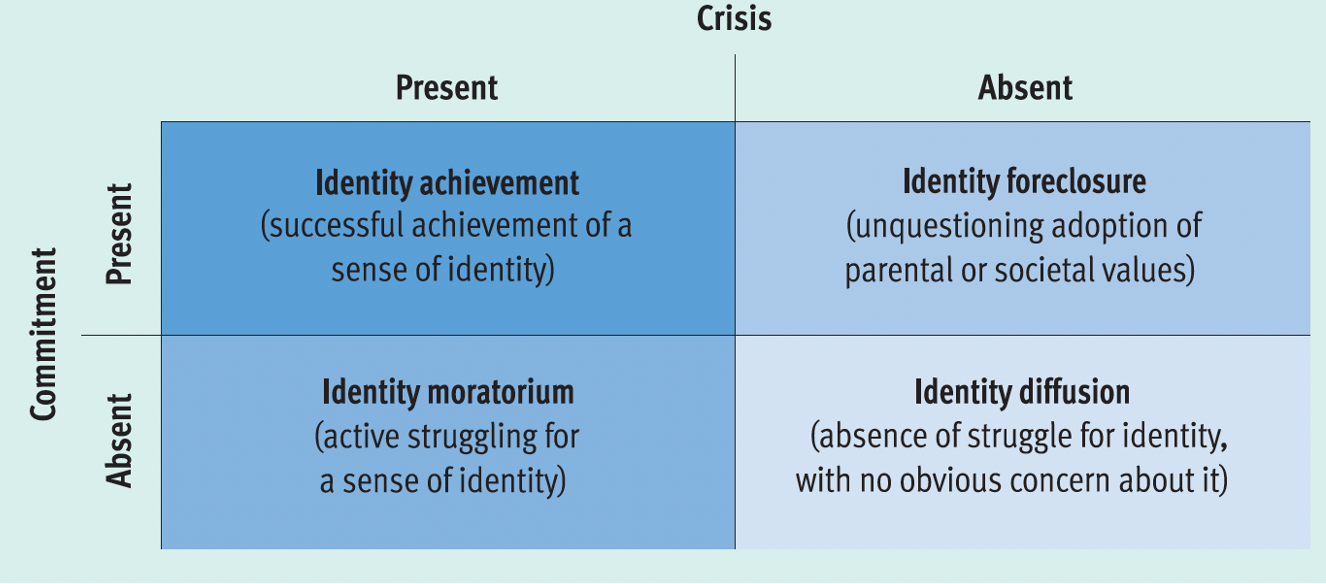
\includegraphics{figs/marcia.png} Identity achievement is
associated with higher self-esteem, conscientiousness, security,
achievement motivation, and capacity for intimacy (Kroger 2006).
\end{frame}

\section{Negative consequences}\label{negative-consequences}

\begin{frame}{Identity confusion might lead to}
\phantomsection\label{identity-confusion-might-lead-to}
(Côté 2018)

\begin{itemize}[<+->]
\tightlist
\item
  Anxiety
\item
  Depression
\item
  Stress and feeling of being overwhelmed
\item
  Generally, not a disorder, unless it becomes debilitating
\item
  For us, it is a bit more complex.
\end{itemize}
\end{frame}

\begin{frame}
\textbf{Have you been in a condition that people don't believe that you
are a New Zealander?}
\end{frame}

\section{Identity denial}\label{identity-denial}

\begin{frame}{Identity denial}
\phantomsection\label{identity-denial-1}
\begin{itemize}[<+->]
\tightlist
\item
  Where are you \emph{really} from?: Asian Americans and identity denial
  (Cheryan and Monin 2005)
\item
  Leads to poor psychological health and wellbeing, such as depressive
  symptoms and stress (Albuja, Sanchez, and Gaither 2019)
\end{itemize}
\end{frame}

\begin{frame}
\textbf{Do you think our youth have an identity problem?}
\end{frame}

\section{Solutions}\label{solutions}

\begin{frame}
\begin{itemize}[<+->]
\tightlist
\item
  Individually: coping, awareness, standing up, promoting positive
  intergroup contact, building bridges
\item
  As a group: nurture a strong supportive social network
\item
  But remember that this should not be exclusive!
\end{itemize}
\end{frame}

\begin{frame}[fragile]{The importance of social support}
\phantomsection\label{the-importance-of-social-support}
\begin{itemize}[<+->]
\tightlist
\item
  Whoever desires an increase in his sustenance and age, should keep
  good relations with kith and kin. \texttt{Sahih\ Muslim}.
\item
  Broad. But comes from family, relatives, friends and peers.
\item
  Social support domains: emotional, instrumental, informational, and
  physical affection. These buffer individuals from stressors.
\item
  Offering/giving social support is more beneficial than receiving it:
  reduces distress, and improves physical as well as mental health.
\item
  In married couples, mortality was significantly reduced for those who
  reported providing instrumental support to friends, relatives,
  neighbours, and spouses (Utz 2011).
\end{itemize}
\end{frame}

\begin{frame}{The importance of family/parenting}
\phantomsection\label{the-importance-of-familyparenting}
\begin{itemize}[<+->]
\tightlist
\item
  Married couples have high emotional, psychological, and physical
  wellbeing
\item
  Reported being more happy
\item
  Significantly low levels of depression
\item
  Children that grow up in a married two parent family are less likely
  to experience emotional-behavioural problems (Brown 2004)
\item
  They are less likely to drop out of the school, use drugs, give birth
  as teenagers, or experience child abuse (Flewelling and Bauman 1990)
\item
  More educated and better educational outcomes (Haurin 1992).
\end{itemize}
\end{frame}

\begin{frame}{What are your thoughts on the following?}
\phantomsection\label{what-are-your-thoughts-on-the-following}
\begin{itemize}[<+->]
\tightlist
\item
  What brought us together here today?
\item
  Do we need to look further into Muslim lives, in a more objective way?
\item
  Are Muslims' happiness, sense of meaning in life, and levels of
  psychological stress similar to those of people from other religious
  groups because of the support they get from their religious
  communities?
\item
  Will attending mosque more, prevent us from feeling of discrimination?
\item
  Do we face more challenges to employment and health service than other
  groups?
\end{itemize}
\end{frame}

\begin{frame}
\begin{enumerate}
\item
  Muslims with the strongest ties to their community as measured by
  service attendance and prayer are buffered most from anti-Muslim
  prejudice.
\item
  Muslims experience greater challenges to employment and health than
  matched members of other religious groups.
\item
  Subjective well-being, the meaning of life, and psychological distress
  are similar among Muslims and matched members of religious groups from
  the buffering of religious community-making.
\end{enumerate}
\end{frame}

\begin{frame}
\begin{figure}

\begin{minipage}{\linewidth}
\begin{center}

\includegraphics[width=0.6\textwidth,height=\textheight]{figs/mds.png}
\end{center}
\end{minipage}%
\newline
\begin{minipage}{\linewidth}

\includegraphics{figs/sponsors.png}\end{minipage}%

\end{figure}%
\end{frame}

\begin{frame}{Our research into the perception of Muslim community
(2016-present)}
\phantomsection\label{our-research-into-the-perception-of-muslim-community-2016-present}
\begin{itemize}[<+->]
\tightlist
\item
  Perception of Muslims in New Zealand
\item
  National identity
\item
  Change in attitudes post March 15 attacks
\end{itemize}
\end{frame}

\begin{frame}[fragile]{My concerns\ldots{}}
\phantomsection\label{my-concerns}
\begin{itemize}
\tightlist
\item
  It does not raise the Muslim voice, because\ldots.
\item
  Muslims are under-represented as \texttt{participants} as well as as
  \texttt{researchers}.
\item
  We don't have an objective understanding of Muslim lives in New
  Zealand.
\end{itemize}
\end{frame}

\section{Muslim Diversity Study}\label{muslim-diversity-study}

\begin{frame}{Muslim Diversity Study covers}
\phantomsection\label{muslim-diversity-study-covers}
\begin{itemize}[<+->]
\tightlist
\item
  Muslims self-perception, perception of discrimination, diversity,
  flourishing, wellbeing, meaning-making, resilience, life satisfaction,
  and health outcomes.
\item
  Effects of religion and religious support.
\end{itemize}
\end{frame}

\begin{frame}{Aims}
\phantomsection\label{aims}
\begin{itemize}[<+->]
\tightlist
\item
  Increase Muslim community \textbf{representation} in research
\item
  Increase \textbf{research opportunities} for the Muslim community
\item
  \textbf{Share findings} back with the community members, leadership,
  and government.
\end{itemize}
\end{frame}

\begin{frame}{FAQ's}
\phantomsection\label{faqs}
\begin{itemize}[<+->]
\tightlist
\item
  Are my responses confidential?
\item
  Can my responses be linked back to me?
\item
  How does it help Muslim community in the long run?
\item
  How can you participate?
\end{itemize}
\end{frame}

\begin{frame}{MDS Team Christchurch}
\phantomsection\label{mds-team-christchurch}
\begin{itemize}
\tightlist
\item
  Marzia Ehsani
\item
  Zahra Haidary
\item
  Khadija Jasim
\item
  Sarah Quader
\end{itemize}
\end{frame}

\begin{frame}{MDS Auckland Team}
\phantomsection\label{mds-auckland-team}
\begin{itemize}
\tightlist
\item
  Omer Anwarzada
\item
  Ayyan Ali
\item
  Asem Arif
\item
  Weaam Bassiouni
\item
  Aqsa Butt
\item
  Dr Iman Hussain
\item
  Abduallah Kalantan
\item
  Noor Najm
\end{itemize}
\end{frame}

\begin{frame}{MDS Hamilton Team}
\phantomsection\label{mds-hamilton-team}
\begin{itemize}
\tightlist
\item
  Sana Nisar Ahmad
\item
  Dr Hala Burhoum
\item
  Yasir Saifudeen
\end{itemize}
\end{frame}

\begin{frame}{MDS Palmerston North Team}
\phantomsection\label{mds-palmerston-north-team}
\begin{itemize}
\tightlist
\item
  Mashal Khan
\end{itemize}
\end{frame}

\begin{frame}{MDS Wellington Team}
\phantomsection\label{mds-wellington-team}
\begin{itemize}
\tightlist
\item
  Tuba Azeem
\item
  Parus Khoso
\item
  Hawwa Niyaz
\item
  Hussain Raissi
\end{itemize}
\end{frame}

\begin{frame}{MDS Dunedin Team}
\phantomsection\label{mds-dunedin-team}
\begin{itemize}
\tightlist
\item
  Dr Farah Shawkat
\item
  Dr Mai Tamimi
\end{itemize}
\end{frame}

\begin{frame}{MDS Media and Admin Team}
\phantomsection\label{mds-media-and-admin-team}
\begin{itemize}
\tightlist
\item
  Jamila Badis
\item
  Noor Najm
\end{itemize}
\end{frame}

\begin{frame}{MDS Core Team}
\phantomsection\label{mds-core-team}
\begin{figure}

\begin{minipage}{0.40\linewidth}
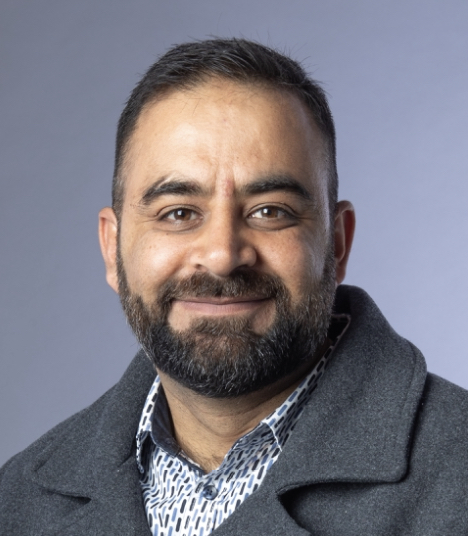
\includegraphics[width=0.9in,height=\textheight]{figs/usman-a.jpeg}\end{minipage}%
%
\begin{minipage}{0.20\linewidth}
~\end{minipage}%
%
\begin{minipage}{0.40\linewidth}
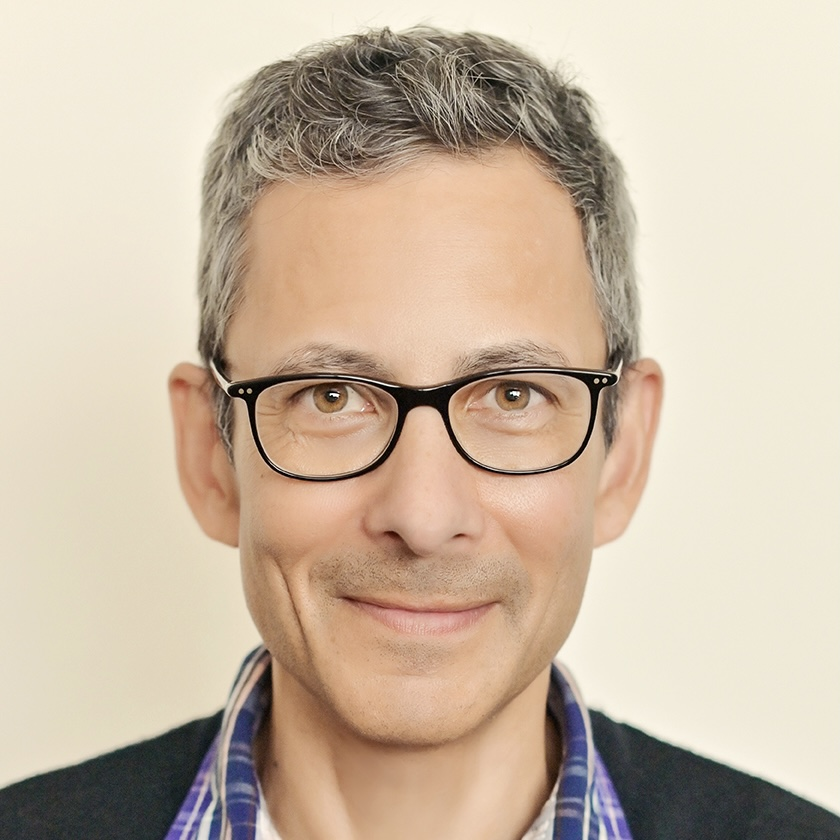
\includegraphics[width=0.9in,height=\textheight]{figs/joe-b.jpg}\end{minipage}%
\newline
\begin{minipage}{0.30\linewidth}
~\end{minipage}%
%
\begin{minipage}{0.40\linewidth}
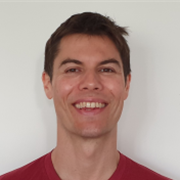
\includegraphics[width=0.9in,height=\textheight]{figs/chris-s.png}\end{minipage}%
%
\begin{minipage}{0.30\linewidth}
~\end{minipage}%
\newline
\begin{minipage}{0.40\linewidth}
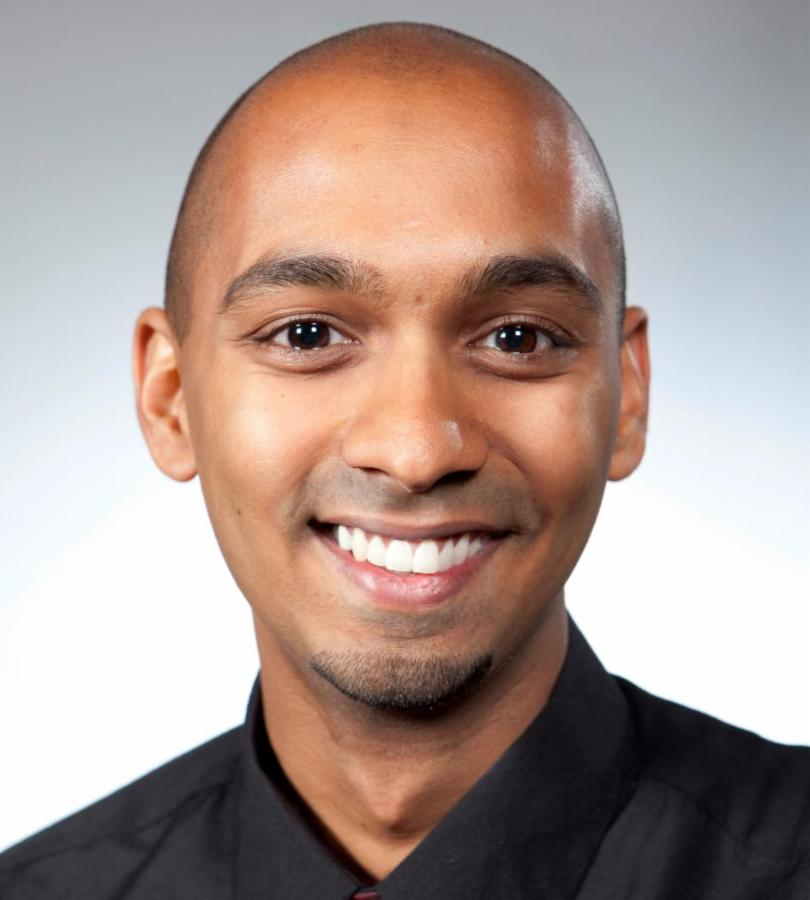
\includegraphics[width=0.9in,height=\textheight]{figs/kumar-y.jpg}\end{minipage}%
%
\begin{minipage}{0.20\linewidth}
~\end{minipage}%
%
\begin{minipage}{0.40\linewidth}
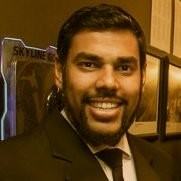
\includegraphics[width=0.9in,height=\textheight]{figs/aarif-r.jpeg}\end{minipage}%

\end{figure}%
\end{frame}

\begin{frame}
\begin{itemize}
\tightlist
\item
  20+ Research Assistants
\item
  Numerous research collaborators
\item
  Muslim Reference Group
\end{itemize}
\end{frame}

\begin{frame}{Talks in the past}
\phantomsection\label{talks-in-the-past}

\includegraphics[width=0.4\textwidth,height=\textheight]{figs/care-lecture.png}


\includegraphics[width=0.4\textwidth,height=\textheight]{figs/uc-lecture.png}
\end{frame}

\begin{frame}{To find out more}
\phantomsection\label{to-find-out-more}

\includegraphics[width=0.5\textwidth,height=\textheight]{figs/mds-uc-banner.png}

\url{https://linktr.ee/muslimdiversity}
\end{frame}

\begin{frame}{Or use this QR code}
\phantomsection\label{or-use-this-qr-code}

\includegraphics[width=0.5\textwidth,height=\textheight]{figs/mds-qr.png}
\end{frame}

\begin{frame}{Thank you}
\phantomsection\label{thank-you}
\begin{itemize}
\tightlist
\item
  UCMUSA
\item
  Christchurch MDS Team
\item
  Asturlab Cultural Centre
\end{itemize}
\end{frame}

\begin{frame}
\textbf{Any questions?}
\end{frame}

\begin{frame}{References}
\phantomsection\label{references}
\phantomsection\label{refs}
\begin{CSLReferences}{1}{0}
\bibitem[\citeproctext]{ref-albuja2019identity}
Albuja, Analia F, Diana T Sanchez, and Sarah E Gaither. 2019.
{``Identity Denied: Comparing American or White Identity Denial and
Psychological Health Outcomes Among Bicultural and Biracial People.''}
\emph{Personality and Social Psychology Bulletin} 45 (3): 416--30.

\bibitem[\citeproctext]{ref-bosson2006}
Bosson, JENNIFER K., AMBER B. JOHNSON, KATE NIEDERHOFFER, and WILLIAM B.
SWANN. 2006. {``Interpersonal Chemistry Through Negativity: Bonding by
Sharing Negative Attitudes about Others.''} \emph{Personal
Relationships} 13 (2): 135--50.
\url{https://doi.org/10.1111/j.1475-6811.2006.00109.x}.

\bibitem[\citeproctext]{ref-brown2004family}
Brown, Susan L. 2004. {``Family Structure and Child Well-Being: The
Significance of Parental Cohabitation.''} \emph{Journal of Marriage and
Family} 66 (2): 351--67.

\bibitem[\citeproctext]{ref-cheryan2005you}
Cheryan, Sapna, and Benoı̂t Monin. 2005. {``Where Are You Really from?:
Asian Americans and Identity Denial.''} \emph{Journal of Personality and
Social Psychology} 89 (5): 717.

\bibitem[\citeproctext]{ref-cuxf4tuxe92018}
Côté, James E. 2018. {``The Enduring Usefulness of Erikson{'}s Concept
of the Identity Crisis in the 21st Century: An Analysis of Student
Mental Health Concerns.''} \emph{Identity} 18 (4): 251--63.
\url{https://doi.org/10.1080/15283488.2018.1524328}.

\bibitem[\citeproctext]{ref-fein1997a}
Fein, Steven, and Steven J. Spencer. 1997. {``Prejudice as Self-Image
Maintenance: Affirming the Self Through Derogating Others.''}
\emph{Journal of Personality and Social Psychology} 73 (1): 31--44.
\url{https://doi.org/10.1037/0022-3514.73.1.31}.

\bibitem[\citeproctext]{ref-flewelling1990family}
Flewelling, Robert L, and Karl E Bauman. 1990. {``Family Structure as a
Predictor of Initial Substance Use and Sexual Intercourse in Early
Adolescence.''} \emph{Journal of Marriage and the Family}, 171--81.

\bibitem[\citeproctext]{ref-haurin1992patterns}
Haurin, R Jean. 1992. {``Patterns of Childhood Residence and the
Relationship to Young Adult Outcomes.''} \emph{Journal of Marriage and
the Family}, 846--60.

\bibitem[\citeproctext]{ref-kroger2006identity}
Kroger, Jane. 2006. {``Identity Development During Adolescence.''}
\emph{Blackwell Handbook of Adolescence}, 205--26.

\bibitem[\citeproctext]{ref-utz2011psychology}
Utz, Aisha. 2011. \emph{Psychology from the Islamic Perspective}.

\bibitem[\citeproctext]{ref-weaver2011}
Weaver, Jonathan R., and Jennifer K. Bosson. 2011. {``I Feel Like I Know
You: Sharing Negative Attitudes of Others Promotes Feelings of
Familiarity.''} \emph{Personality and Social Psychology Bulletin} 37
(4): 481--91. \url{https://doi.org/10.1177/0146167211398364}.

\end{CSLReferences}
\end{frame}



\end{document}
